%%%%%%%%%%%%%%%%%%%%%%%%%%%%%%%%%%%%%%%%%%%%%%%%%%%%%%%%%%%%%%%%%%%%%%
%%  Copyright by Wenliang Du.                                       %%
%%  This work is licensed under the Creative Commons                %%
%%  Attribution-NonCommercial-ShareAlike 4.0 International License. %%
%%  To view a copy of this license, visit                           %%
%%  http://creativecommons.org/licenses/by-nc-sa/4.0/.              %%
%%%%%%%%%%%%%%%%%%%%%%%%%%%%%%%%%%%%%%%%%%%%%%%%%%%%%%%%%%%%%%%%%%%%%%

\newcommand{\commonfolder}{../../common-files}

\documentclass[11pt]{article}

\usepackage[most]{tcolorbox}
\usepackage{times}
\usepackage{epsf}
\usepackage{epsfig}
\usepackage{amsmath, alltt, amssymb, xspace}
\usepackage{wrapfig}
\usepackage{fancyhdr}
\usepackage{url}
\usepackage{verbatim}
\usepackage{fancyvrb}
\usepackage{adjustbox}
\usepackage{listings}
\usepackage{color}
\usepackage{subfigure}
\usepackage{cite}
\usepackage{sidecap}
\usepackage{pifont}
\usepackage{mdframed}
\usepackage{textcomp}
\usepackage{enumitem}
\usepackage{hyperref}


% Horizontal alignment
\topmargin      -0.50in  % distance to headers
\oddsidemargin  0.0in
\evensidemargin 0.0in
\textwidth      6.5in
\textheight     8.9in 

\newcommand{\todo}[1]{
\vspace{0.1in}
\fbox{\parbox{6in}{TODO: #1}}
\vspace{0.1in}
}


\newcommand{\unix}{{\tt Unix}\xspace}
\newcommand{\linux}{{\tt Linux}\xspace}
\newcommand{\minix}{{\tt Minix}\xspace}
\newcommand{\ubuntu}{{\tt Ubuntu}\xspace}
\newcommand{\setuid}{{\tt Set-UID}\xspace}
\newcommand{\openssl} {\texttt{openssl}}

% Arrows
\newcommand{\pointleft}[1]{\reflectbox{\ding{217}} \textbf{\texttt{#1}}}
\newcommand{\pointright}[1]{\ding{217} \textbf{\texttt{#1}}}
\newcommand{\pointupleft}[1]{\reflectbox{\ding{218}} \textbf{\texttt{#1}}}

% Line numbers
\newcommand{\lineone}{\ding{192}\xspace}
\newcommand{\linetwo}{\ding{193}\xspace}
\newcommand{\linethree}{\ding{194}\xspace}
\newcommand{\linefour}{\ding{195}\xspace}
\newcommand{\linefive}{\ding{196}\xspace}
\newcommand{\linesix}{\ding{197}\xspace}
\newcommand{\lineseven}{\ding{198}\xspace}
\newcommand{\lineeight}{\ding{199}\xspace}
\newcommand{\linenine}{\ding{200}\xspace}


% Fancy headers
\pagestyle{fancy}
\lhead{\bfseries SEED Labs}
\chead{}
\rhead{\small \thepage}
\lfoot{}
\cfoot{}
\rfoot{}


\definecolor{dkgreen}{rgb}{0,0.6,0}
\definecolor{gray}{rgb}{0.5,0.5,0.5}
\definecolor{mauve}{rgb}{0.58,0,0.82}
\definecolor{lightgray}{gray}{0.90}


\lstset{%
  frame=none,
  language=,
  backgroundcolor=\color{lightgray},
  aboveskip=3mm,
  belowskip=3mm,
  showstringspaces=false,
%  columns=flexible,
  basicstyle={\small\ttfamily},
  numbers=none,
  numberstyle=\tiny\color{gray},
  keywordstyle=\color{blue},
  commentstyle=\color{dkgreen},
  stringstyle=\color{mauve},
  breaklines=true,
  breakatwhitespace=true,
  tabsize=3,
  columns=fullflexible,
  keepspaces=true,
  escapeinside={(*@}{@*)}
}

\newcommand{\newnote}[1]{
\vspace{0.1in}
\noindent
\fbox{\parbox{1.0\textwidth}{\textbf{Note:} #1}}
%\vspace{0.1in}
}


%% Submission
\newcommand{\seedsubmission}{You need to submit a detailed lab report, with screenshots,
to describe what you have done and what you have observed.
You also need to provide explanation
to the observations that are interesting or surprising.
Please also list the important code snippets followed by
explanation. Simply attaching code without any explanation will not
receive credits.}

%% Book
\newcommand{\seedbook}{\textit{Computer \& Internet Security: A Hands-on Approach}, 3rd
Edition, by Wenliang Du. See details at \url{https://www.handsonsecurity.net}.\xspace}

\newcommand{\seedisbook}{\textit{Internet Security: A Hands-on Approach}, 3rd
Edition, by Wenliang Du. See details at \url{https://www.handsonsecurity.net}.\xspace}

\newcommand{\seedcsbook}{\textit{Computer Security: A Hands-on Approach}, 3rd
Edition, by Wenliang Du. See details at \url{https://www.handsonsecurity.net}.\xspace}

\newcommand{\seedcibook}{\textit{Computer \& Internet Security: A Hands-on Approach}, 3rd
Edition, by Wenliang Du. See details at \url{https://www.handsonsecurity.net}.\xspace}

%% Videos
\newcommand{\seedisvideo}{\textit{Internet Security: A Hands-on Approach},
by Wenliang Du. See details at \url{https://www.handsonsecurity.net/video.html}.\xspace}

\newcommand{\seedcsvideo}{\textit{Computer Security: A Hands-on Approach},
by Wenliang Du. See details at \url{https://www.handsonsecurity.net/video.html}.\xspace}

%% Lab Environment
\newcommand{\seedenvironment}{This lab has been tested on our pre-built
Ubuntu 16.04 VM, which can be downloaded from the SEED website.\xspace}

\newcommand{\seedenvironmentA}{This lab has been tested on our pre-built
Ubuntu 16.04 VM, which can be downloaded from the SEED website.\xspace}

\newcommand{\seedenvironmentB}{This lab has been tested on our pre-built
Ubuntu 20.04 VM, which can be downloaded from the SEED website.\xspace}

\newcommand{\seedenvironmentC}{This lab has been tested on the SEED
Ubuntu 20.04 VM. You can download a pre-built image from the SEED website, 
and run the SEED VM on your own computer. However,
most of the SEED labs can be conducted on the cloud, and 
you can follow our instruction to create a SEED VM on the cloud.\xspace}

\newcommand{\seedenvironmentAB}{This lab has been tested on our pre-built
Ubuntu 16.04 and 20.04 VMs, which can be downloaded from the SEED website.\xspace}

\newcommand{\nodependency}{Since we use containers to set up the lab environment, 
this lab does not depend much on the SEED VM. You can do this lab
using other VMs, physical machines, or VMs on the cloud.\xspace}

\newcommand{\adddns}{You do need to add the required IP address mapping to
the \texttt{/etc/hosts} file.\xspace}






\newcommand{\seedlabcopyright}[1]{
\vspace{0.1in}
\fbox{\parbox{6in}{\small Copyright \copyright\ {#1}\ \ by Wenliang Du.\\
      This work is licensed under a Creative Commons
      Attribution-NonCommercial-ShareAlike 4.0 International License.
      If you remix, transform, or build upon the material, 
      this copyright notice must be left intact, or reproduced in a way that is reasonable to
      the medium in which the work is being re-published.}}
\vspace{0.1in}
}




\hypersetup{%
    pdfborder = {0 0 0}
}

\lhead{\bfseries SEED Labs -- DNS Infrastructure}
\newcommand{\dnsFigs}{./Figs}


\usepackage{hyperref}

\begin{document}


\begin{center}
{\LARGE DNS Infrastructure Lab}
\end{center}

\seedlabcopyright{2021}



% *******************************************
% SECTION
% ******************************************* 
\section{Overview}

DNS (Domain Name System) is the Internet's phone book; it
translates hostnames to IP addresses (and vice versa).
This translation is through DNS resolution, which happens behind
the scene. The resolution process involves many nameservers,
including root servers, TLD servers, and final domain servers.
These nameservers form the entire DNS system, which is an
essential infrastructure for the Internet.

To help students understand how these nameservers work together
to form the infrastructure, we will create a miniature DNS system
inside an Internet Emulator.
Even though this system is small, it has all the essential
elements of a real DNS infrastructure. By building such a system,
students will have a deeper understanding of how the DNS actually works.
Although this lab is not a security lab, it is the basis for
several SEED labs. This lab covers the following topics:

\begin{itemize}[noitemsep]
\item The DNS infrastructure
\item DNS forward and reverse lookup processes
\item Root and TLD servers
\item DNS resolver, local DNS server
\end{itemize}



\paragraph{Readings and videos.}
Detailed coverage of the DNS protocol can be found in the following:

\begin{itemize}
\item Chapter 23 of the SEED Book, \seedcibook
\item Chapter 10 of the SEED Book, \seedisbook
\item Section 7 of the SEED Lecture, \seedisvideo
\end{itemize}


\paragraph{Lab environment.} 
\seedenvironmentB
\nodependency

\paragraph{Overview of the lab tasks.}
The DNS infrastructure involves many servers. We will
build a simplified DNS infrastructure inside the emulator. 
This infrastructure includes two root servers, two \texttt{com}
TLD (Top-Level Domain) servers, one \texttt{edu} TLD server,
and two second-level domain nameservers (See 
Figure~\ref{dns:fig:dns-infrastructure}). It should be noted 
that students need to replace \texttt{smith2021} with their 
own last names and the present year. 


\begin{figure}[htb]
  \begin{center}
    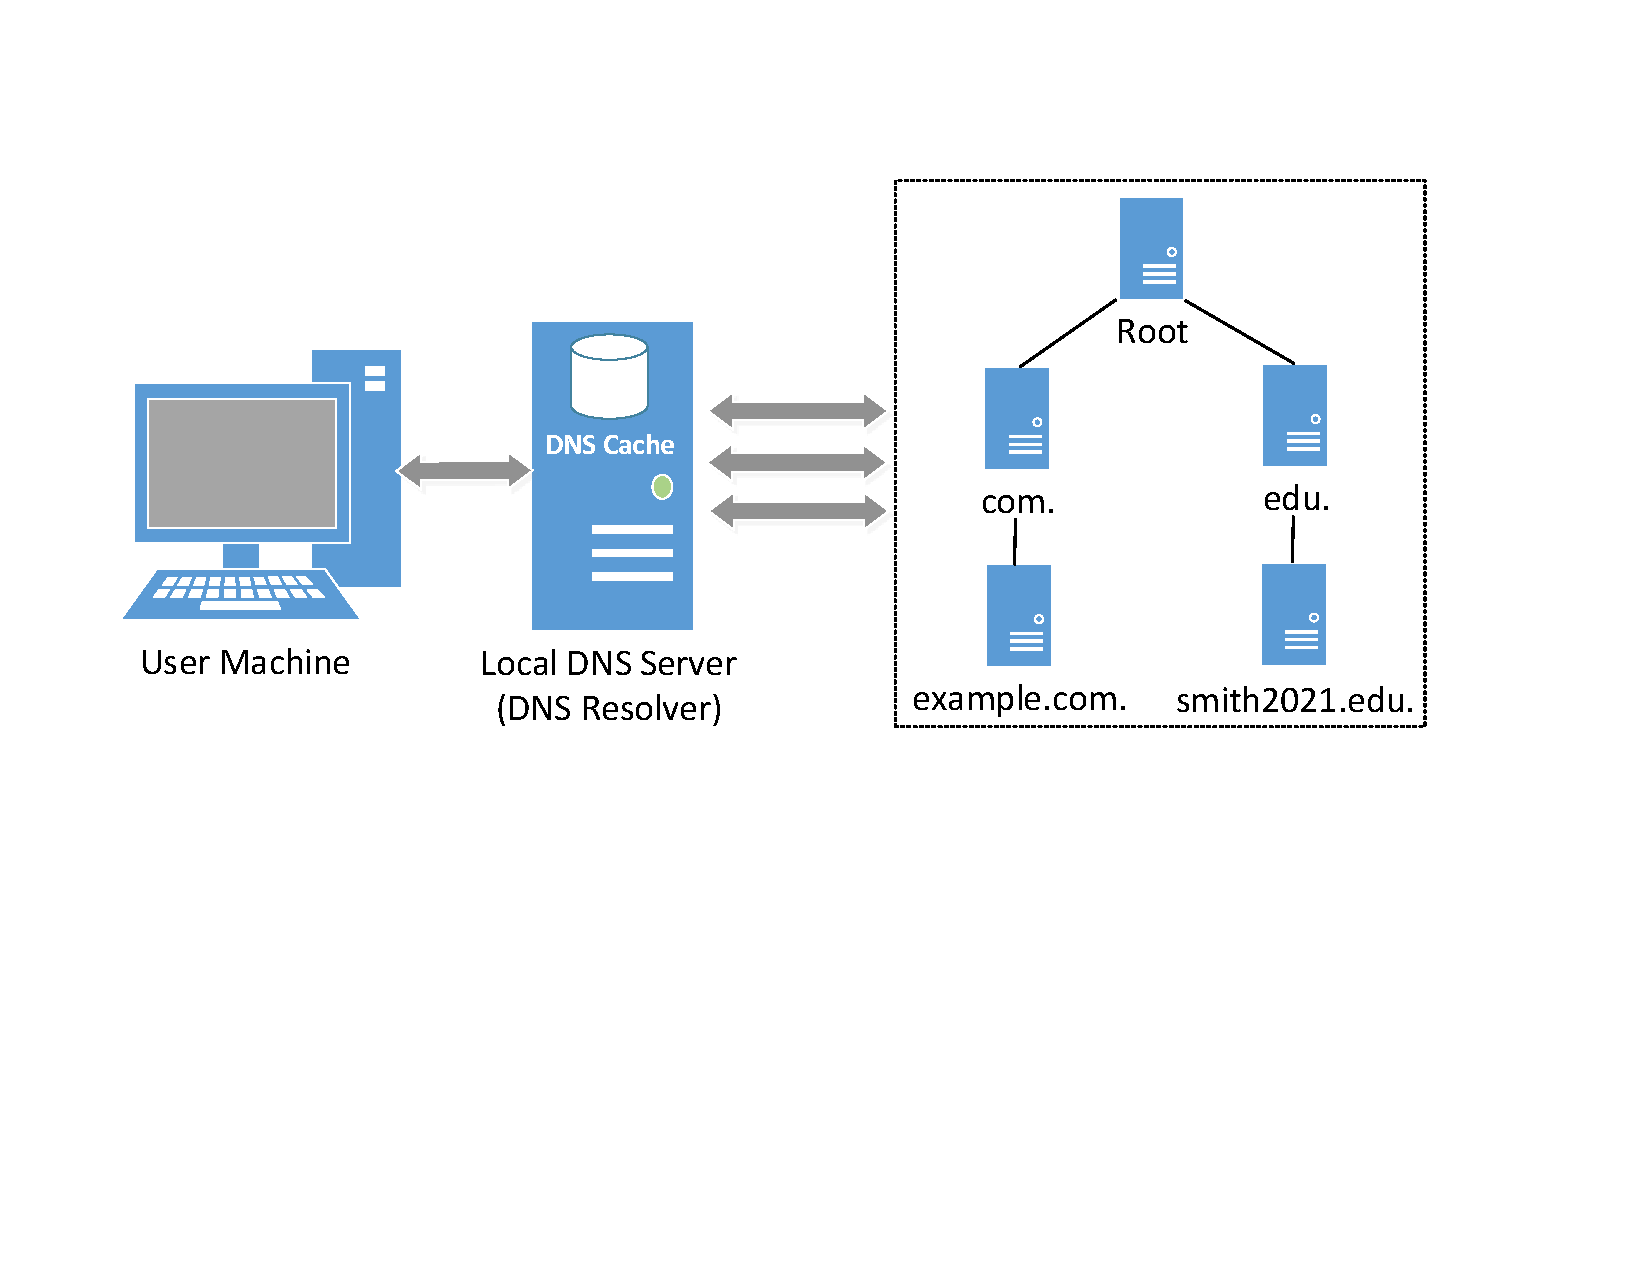
\includegraphics[width=0.7\textwidth]{\dnsFigs/dns_infrastructure.pdf}
  \end{center}
  \caption{The simplified DNS Infrastructure}
  \label{dns:fig:dns-infrastructure}
\end{figure}

We need to configure the nameservers for each of the zone
depicted in the figure. We will do it from the bottom up.
Namely, we will configure the second-level domain nameservers
first (Task 1), then the TLD server (Task 2), and 
then the Root server (Task 3). We also need to configure
the local DNS server and the client machine (Tasks 4 and 5), 
so the client machine can use the DNS infrastructure. 
Task 6 is to complete the DNS infrastructure for the reverse 
lookup.


% -------------------------------------------
% SUBSECTION
% -------------------------------------------
\section{The Lab Setup and the SEED Internet Emulator}

This lab will be performed inside the SEED Internet Emulator (simply
called the emulator in this document). If this is the first time you
use the emulator, it is important that you read this section. 
We recommend instructors to provide a lab session to 
help students get familiar with the emulator.  


% -------------------------------------------
% SUBSECTION
% -------------------------------------------
\subsection{The Internet Emulator} 


We provide a pre-built emulator in two different forms: Python code
and container files. The container files are generated from
the Python code, but students need to install the SEED Emulator source
code from the GitHub to run the Python code. The container files
can be directly used without the emulator source code.
Instructors who would like to customize the emulator can modify the Python
code, generate their own container files, and then provide the
files to students, replacing the ones included in the
lab setup file. See the \texttt{README.md} file for instructions. 


\paragraph{Download the emulator files.}
Please download the \texttt{Labsetup.zip} file from the web page, and
unzip it. The files inside the container folder are the actual 
emulation files (container files); they are generated by the Python code.
The name of the container folder is called \texttt{output/} for most labs,
but if a lab has multiple emulators, it will use 
different folder names. The actual names will be given in the lab task.


\paragraph{Start the emulation.}
We will directly use the files in the container folder.
Go to this folder, and run the docker commands
to build and start the containers. We recommend that you run the emulator inside
the provided SEED Ubuntu 20.04 VM, but doing it in a generic Ubuntu 20.04 operating system
should not have any problem, as long as the docker software is installed.
Readers can find the docker manual from
\href{https://github.com/seed-labs/seed-labs/blob/master/manuals/docker/SEEDManual-Container.md}
{\underline{this link}}.
If this is the first time you set up a SEED lab environment
using containers, it is very important that you read 
the user manual. 


In the following, we list some of the commonly
used commands related to Docker and Compose. 
Since we are going to use 
these commands very frequently, we have created aliases for them
in the \texttt{.bashrc} file (in our provided SEEDUbuntu 20.04 VM).

\begin{lstlisting}
$ docker-compose build  # Build the container images
$ docker-compose up     # Start the containers
$ docker-compose down   # Shut don the containers


// Aliases for the Compose commands above
$ dcbuild       # Alias for: docker-compose build
$ dcup          # Alias for: docker-compose up
$ dcdown        # Alias for: docker-compose down
\end{lstlisting}


All the containers will be running in the background. To run
commands on a container, we often need to get a shell on
that container. We first need to use the \texttt{"docker ps"}  
command to find out the ID of the container, and then
use \texttt{"docker exec"} to start a shell on that 
container. We have created aliases for them in
the \texttt{.bashrc} file.

\begin{lstlisting}
$ dockps        // Alias for: docker ps --format "{{.ID}}  {{.Names}}" 
$ docksh <id>   // Alias for: docker exec -it <id> /bin/bash

// The following example shows how to get a shell inside hostC
$ dockps
b1004832e275  hostA-10.9.0.5
0af4ea7a3e2e  hostB-10.9.0.6
9652715c8e0a  hostC-10.9.0.7

$ docksh 96
root@9652715c8e0a:/#  

// Note: If a docker command requires a container ID, you do not need to 
//       type the entire ID string. Typing the first few characters will 
//       be sufficient, as long as they are unique among all the containers. 
\end{lstlisting}


If you encounter problems when setting up the lab environment, 
please read the ``Common Problems'' section of the manual
for potential solutions.



\paragraph{Set the terminal title.} 
We may need to get into several containers using the terminal.
We will likely create several terminal tabs, and switch back
and forth among these tabs. We can easily get lost, because
it is difficult to know which tab runs which container. 
To solve this problem, once we
are inside a container, we can set the terminal title using
one of the following commands (it sets the title to \texttt{"New Title"}).

\begin{lstlisting}
# set_title New Title
# st New Title       (*@\pointleft{st} is an alias of set\_title@*)
\end{lstlisting}






% -------------------------------------------
% SUBSECTION
% -------------------------------------------
\subsection{The Map of the Emulated Internet} 



% The actual figure file is inside common-files/Figs/. Therefore, 
% when this file is inclucded in another tex file located in folder A, 
% a symbolic link should be created inside A/Figs to link the filename
% to the actual figure file inside the common-files/Figs/ folder.
\begin{figure}[htb]
  \begin{center}
    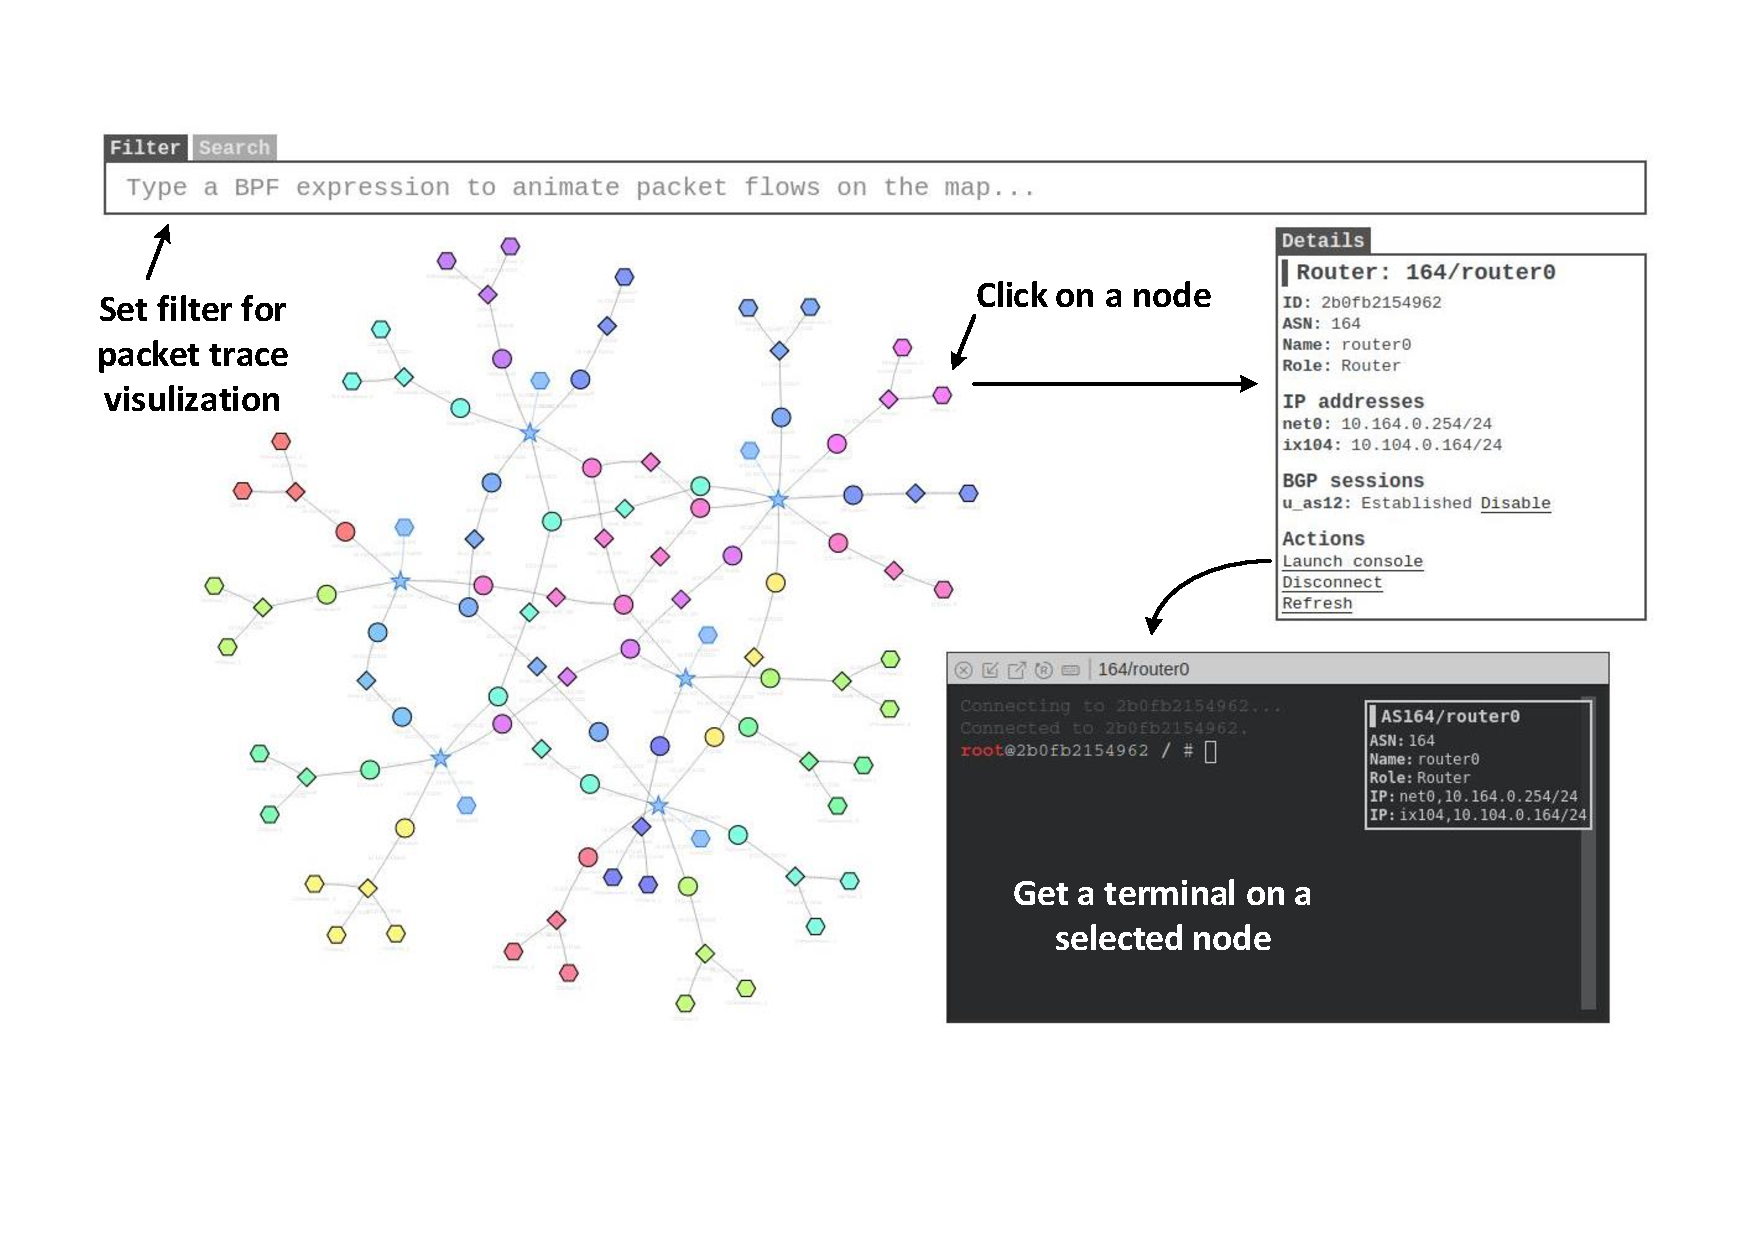
\includegraphics[width=0.95\textwidth]{./Figs/emulator_gui.pdf}
  \end{center}
  \caption{The map of the emulated Internet}
  \label{emulator:fig:emulator-gui}
\end{figure}


Each computer (hosts or routers) running inside the emulator is a docker container.
Users can access these computers using docker commands, such as getting a shell
inside a container.
The emulator also comes with a web application, which visualizes all the hosts, routers,
and networks.
After the emulator starts, the map can be accessed from this
URL: \url{http://localhost:8080/map.html}.
See Figure~\ref{emulator:fig:emulator-gui}.
To zoom in/out, use the mouse middle scroll. 
Click on any node, the detailed information of that node
will be displayed on the side panel, from where,
users can get a console on that node (container). 








% -------------------------------------------
% SUBSECTION
% -------------------------------------------
\subsection{Filtering and Replying} 




% The actual figure file is inside common-files/Figs/. Therefore, 
% when this file is inclucded in another tex file located in folder A, 
% a symbolic link should be created inside A/Figs to link the filename
% to the actual figure file inside the common-files/Figs/ folder.
\begin{figure}[htb]
  \begin{center}
        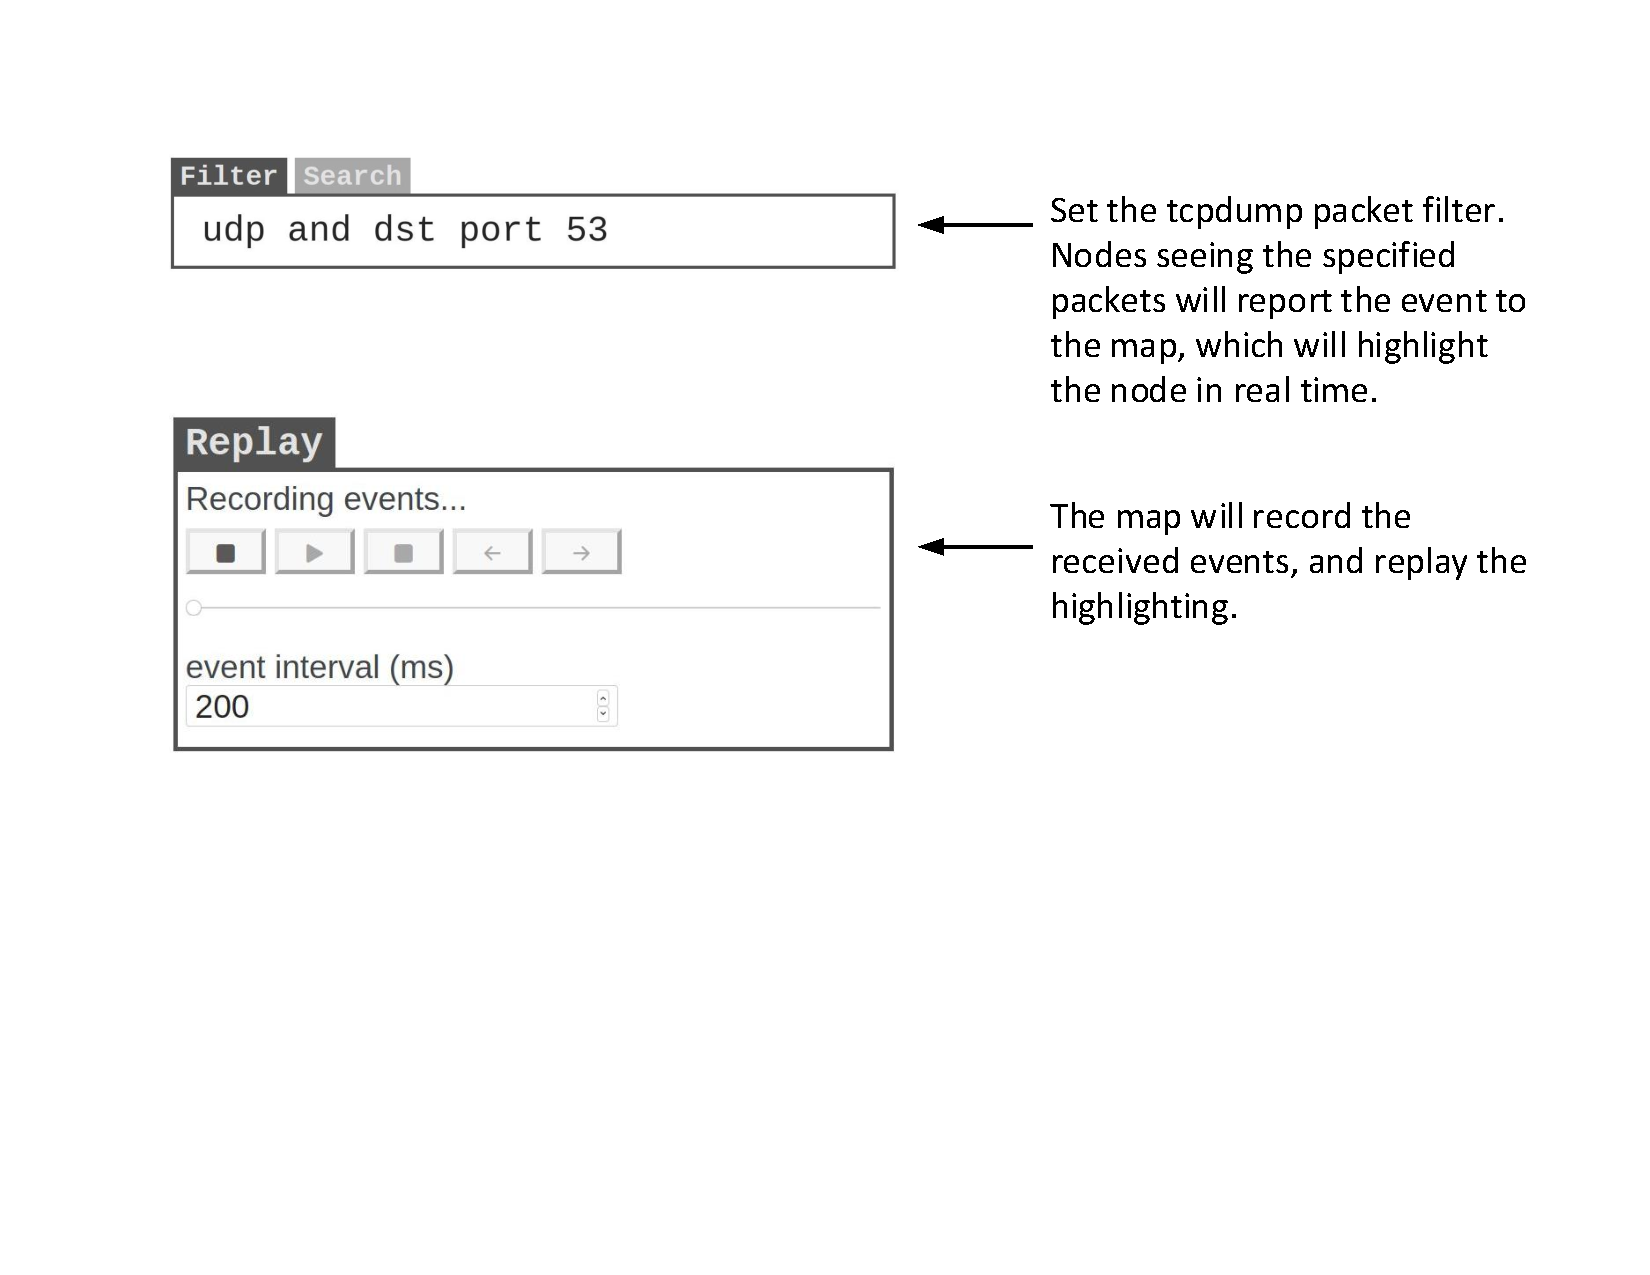
\includegraphics[width=0.6\textwidth]{./Figs/emulator_filter_replay.pdf}
  \end{center}
  \caption{Capturing and replaying events}
  \label{emulator:fig:replay-event}
\end{figure}

Users can also set filters to visualize network traffic.
The syntax of the filter is the same as that in \texttt{tcpdump}; actually,
the filter is directly fed into the \texttt{tcpdump} program running on all nodes.
When a node sees the packets that satisfy the filter, it 
sends an event to the map, which will highlight the node briefly on
the map. 

Sometimes, a sequence of events happen too fast to see the actual order 
among them. In this case, we can use the Replay panel (see 
Figure~\ref{emulator:fig:replay-event}) to record the events and then
replay them at a slower pace. The speed of replaying can be 
adjusted by changing the event interval.





% -------------------------------------------
% SUBSECTION
% -------------------------------------------
\subsection{All the Nameservers} 

In this emulator, the DNS infrastructure is formed 
by a number of the containers running DNS nameservers. 
We have customized their container names, so they can be easily found.
All of the containers have the term
\texttt{DNS} in their names, and their IP addresses 
are also included in the names. 
The following command can list all of them (the
order is re-arranged for the displaying purpose). 

\begin{lstlisting}
$ dockps | grep DNS
dedc6676421e  as150h-DNS-Root-A-10.150.0.72
de5dc343224f  as160h-DNS-Root-B-10.160.0.72
84cf7c7f337d  as151h-DNS-COM-A-10.151.0.72
20c134dceee4  as161h-DNS-COM-B-10.161.0.72
f20fe7ed115f  as152h-DNS-EDU-10.152.0.71
cfabce676bed  as154h-DNS-Example-10.154.0.71
5801404d45d2  as162h-DNS-AAAAA-10.162.0.72
c357ff76bda6  as153h-Global_DNS-1-10.153.0.53
d65e76c44437  as163h-Global_DNS-2-10.163.0.53

// Get a shell on a selected container
$ docksh cfab   (*@\pointleft{container ID}@*) 
root@cfabce676bed / #
root@cfabce676bed / # st Example    (*@\pointleft{change the terminal title}@*)
\end{lstlisting}


 

% -------------------------------------------
% SUBSECTION
% -------------------------------------------
\subsection{Copy DNS Zone Files} 

In this lab, we need to modify the DNS zone files (also
some of the configuration files) inside several containers. We can do that
inside those containers. The problem is that once the containers are stopped
and removed, those changes will be lost. It is better to copy those files
to the hosting machine, make change on the host, and then copy them 
back to the container.  We can use the \texttt{"docker cp"} command
to do that. Since we need to run this command very often, we wrote 
the following shell scripts, one for getting a zone file from container
to the host, and the other for copying the zone file back 
to the container. Both files are included in the lab setup folder.

\begin{lstlisting}[caption=Getting the zone file from container: \texttt{getzone.sh}]
#!/bin/bash

keyword=$1   # Command-line argument 1: used to identify container
filename=$2  # Command-line argument 2: zone file name on container
filename_to=${keyword}_${filename}                                  (*@\lineone@*)
containerID=$(docker ps | grep $keyword | awk '{print $1}')         (*@\linetwo@*) 
if [[ ! -f $filename_to ]]; then
   docker cp $containerID:/etc/bind/zones/$filename ./$filename_to  (*@\linethree@*) 
else
   echo "** File $filename_to already exists; will not overwrite."
fi
\end{lstlisting}

In the emulator, zone files are stored inside the \texttt{/etc/bind/zones} folder.  
Each DNS nameservers have a unique keyword in its container name, for example
the nameserver for the \texttt{example.com} zone has the keyword \texttt{Example}
in its name. We use this keyword to find the corresponding container's ID (see
Line~\linetwo). We also prepend the keyword to the name of the zone file, so we can
easily identify them once they are copied to the host machine (see Lines~\lineone
and~\linethree). The following examples show how we get the zone file from
the two root nameservers and the \texttt{example.com} nameserver.  


\begin{lstlisting}
$ ./getzone.sh Root-A root           (*@\pointleft{}@*) New file: Root-A_root
$ ./getzone.sh Root-B root           (*@\pointleft{}@*) New file: Root-B_root
$ ./getzone.sh Example example.com.  (*@\pointleft{}@*) New file: Example_example.com
\end{lstlisting}
 

Copying files back to  the container is quite similar, except that 
we need to restart the nameserver after the zone file is copied (see Line~\linefour).

\begin{lstlisting}[caption=Sending the zone file to container: \texttt{sendzone.sh}]
#!/bin/bash

keyword=$1   # Command-line argument 1: used to identify container
filename=$2  # Command-line argument 2: zone file name on container
filename_from=${keyword}_${filename}
containerID=$(docker ps | grep $keyword | awk '{print $1}')
if [[ -f $filename_from ]]; then
   echo "== Copy zone file to container"
   docker cp ./$filename_from $containerID:/etc/bind/zones/$filename

   echo "== Restart the nameserver"
   docker exec $containerID service named restart      (*@\linefour@*) 
else
   echo "** File $filename_from does not exists."
fi
\end{lstlisting}
 
Here is an example of how to use \texttt{sendzone.sh}. It sends the 
Root-A's zone file (\texttt{Root-A\_root}) back to Root-A's container,
and restart the nameserver.

\begin{lstlisting}
$ ./sendzone.sh Root-A root
== Copy zone file to container
== Restart the nameserver
 * Stopping domain name service... named
waiting for pid 92 to die
   ...done.
 * Starting domain name service... named
   ...done.
\end{lstlisting}



% *******************************************
% SECTION
% *******************************************
\section{Task 1: Configure the Domain Nameserver}
\label{dns-inf:sec:task1}

In this task, we will configure the nameservers 
for two domains, one is \texttt{example.com}, 
and the other is a customized name based on 
student's name. 

% -------------------------------------------
% SUBSECTION
% -------------------------------------------
\subsection{Task 1.a: Configure the Nameserver for \texttt{example.com}} 

In this task, we will configure the nameserver for a domain
called \texttt{example.com}. The nameserver is hosted on 
one of the containers inside the emulator. The keyword \texttt{Example} is 
included in the container name, as well
as the IP address. 

\begin{lstlisting}
$ dockps | grep Example
46ab89e26738  as154h-DNS-Example-10.154.0.71
\end{lstlisting}


\paragraph{Step 1. Add the zone entry.} 
To host a server for the \texttt{example.com} domain, we need to
add a zone entry to the BIND's configuration, 
so it knows what zones it is going to host. 
In the emulator, the zones hosted by a nameserver are placed 
in the \path{/etc/bind/named.conf.zones} file (multiple zones
can be placed in this file). Here is 
an example, where the \texttt{file} entry specifies
the actual file containing the zone information.  If we want 
to host another zone on this nameserver, we can add a corresponding
zone entry in this file. 

\begin{lstlisting}
zone "example.com" { 
    type master;        (*@\pointleft{this is the master server}@*) 
    allow-update { any; }; 
    file "/etc/bind/zones/example.com.";  (*@\pointleft{the actual zone file}@*) 
};

zone "example.net" {
    ... 
}
\end{lstlisting}


The above entry for the \texttt{example.com} zone 
indicates that the current nameserver
is the master server for this domain, and the zone file is
specified in the \texttt{file} entry.
In the emulator, the zone files are placed inside the 
\path{/etc/bind/zones} folder. It should be noted that 
most of the zone files (except the root zone) have the \texttt{.} 
at the end of the filename. 
This is the main file that we need to modify in this lab. 

\paragraph{Step 2. Modify the zone file.}
Add at least four records (type \texttt{A}) to the zone file
to map hostnames to IP addresses. You can use the 
asterisk (\texttt{*}) as a wildcard hostname. 


\begin{lstlisting}
$TTL 300               (*@\pointleft{The default time to live: 300 seconds}@*) 
$ORIGIN example.com.   (*@\pointleft{The start of this zone file in the namespace}@*) 
@ SOA ns1.example.com. admin.example.com. (*@\textbf{1635647622}@*) 900 900 1800 60

@                  NS    ns1.example.com.
ns1.example.com.   A     10.154.0.71

www                A     10.154.0.72
abc                A     10.154.0.73 
\end{lstlisting}

The zone file must specify the Start of Authority (SOA) record, which
contains the name of the authoritative master name server for the zone, 
the email address of someone responsible for management of the name server,
The parameters of the SOA record also specify a list of timing
and expiration parameters (serial number, slave refresh period, slave retry time, slave
expiration time, and the maximum time to cache the record). 
If we modify the zone file, we should change the serial number (the highlighted 
number in the SOA entry), so the change can be synchronized to the 
slave nameservers. 

In the zone file, domain names that end with a full stop character (i.e., the dot),
are fully qualified while those that do not end with a full stop are
relative to the current origin. 
For example, in the above example, \texttt{ns1.example.com.} is a full name,
while \texttt{www} example refers to \texttt{www.example.com}.


\paragraph{Step 3. Restarting the nameserver.}
Every time we modify the BIND configuration files,
we should to restart the nameserver, so the changes 
can take effect. If there are mistakes in the configuration files,
the nameserver will fail to start.


\begin{lstlisting}
# service named restart
 * Stopping domain name service... named                                                                 waiting for pid 92 to die
                                                                                                  [ OK ]
 * Starting domain name service... named
\end{lstlisting}


\paragraph{Step 4. Testing.} 
Since we have not finished setting up the entire 
DNS infrastructure, we need to 
use the \texttt{@10.154.0.71} option to send our DNS query
directly to \texttt{10.154.0.71}, which is the IP
address of the \texttt{example.com} nameserver in our emulator.
If everything is done correctly, you can get the IP address specified
in your zone file. Please report your observations.

\begin{lstlisting}
$ dig @10.154.0.71 www.example.com
... 
;; ANSWER SECTION:
xyz.example.com.    300    IN    A    (*@\textbf{1.2.3.6}@*)
...
\end{lstlisting}




% -------------------------------------------
% SUBSECTION
% -------------------------------------------
\subsection{Task 1.b: Configure Nameserver for Another Domain} 


In this task, we will configure the nameserver for another domain.
The name of the domain should use the following 
format \texttt{<NAME><YEAR>.edu}, where \texttt{<NAME>} should be 
replaced with your last name, and \texttt{<YEAR>} be replaced 
with the current year. 
For example, if your last name is \texttt{Smith}, and 
it is year 2021, the domain will be \texttt{smith2021.edu}.  
In the emulator, an empty nameserver has already been created;
the keyword \texttt{AAAAA} is encoded in the container name. Please 
use this nameserver to host your domain. 

\begin{lstlisting}
$ dockps | grep AAAAA
70f2e8a57a96  as162h-DNS-AAAAA-10.162.0.72
\end{lstlisting}




% *******************************************
% SECTION
% *******************************************
\section{Task 2: Configure the TLD servers}


In this task, we will configure the nameservers for two TLD domains:
\texttt{com} and \texttt{edu}. We have already created
three nameservers for these two TLD domains. 

\begin{lstlisting}
$ dockps | grep DNS
c3040914667c  as151h-DNS-COM-A-10.151.0.72    (*@\pointleft{The master com server}@*) 
3fa8fa41afb6  as161h-DNS-COM-B-10.161.0.72    (*@\pointleft{The slave com server}@*)
6c7132feb7d4  as152h-DNS-EDU-10.152.0.71      (*@\pointleft{The edu server}@*)
...
\end{lstlisting}
 
There are two nameservers for the \texttt{com} zone. One is configured as 
the master server, and the other as the slave server. 
We only need to modify the zone file on the master (\texttt{COM-A}), 
as the slave server will automatically synchronize 
with the master server. See the following zone configuration
on these two servers. 

\begin{lstlisting}
// For master (COM-A)
zone "com." { type master; allow-transfer { any; }; ...};

// For slave (COM-B)
zone "com." { type slave; masters { 10.151.0.72; }; ... };
\end{lstlisting}


All the nameservers within a TLD domain
must register their nameservers with this
TLD server; otherwise, nobody can find them. 
For each domain, such as \texttt{example.com},  
we need to add two records in the \texttt{com} server's
zone file: an \texttt{NS} record and an \texttt{A} record.
The \texttt{NS} record specifies the nameserver for the
\texttt{example.com} domain, while the \texttt{A} record
specifies the IP address of the nameserver. 


\paragraph{Lab Task.}
Please register your \texttt{example.com} and \texttt{<NAME><YEAR>.edu} 
nameservers with their corresponding TLD servers. Remember to run
\texttt{"service named restart"}  to restart the nameserver after the
changes. Also remember to change the serial number of the zone file; otherwise,
the changes on the master server will not be synchronized to the 
slave server. After making the changes, please run the following commands
to test the servers. 
Report and explain your observations. 

\begin{lstlisting}
# dig @10.151.0.72 www.example.com       (*@\pointleft{Query the COM-A server}@*) 
# dig @10.161.0.72 www.example.com       (*@\pointleft{Query the COM-B server}@*) 
# dig @10.152.0.72 www.<NAME><YEAR>.edu  (*@\pointleft{Query the EDU server}@*) 
\end{lstlisting}



It should be noted, the TLD servers are configured
not to conduct the recursive query, so they will only tell you
the nameserver for the domain name in the query; it will not
resolve the query for you.  See the following configuration.

\begin{lstlisting}
// File: named.conf.options
options {
        directory "/var/cache/bind";
        (*@\textbf{recursion no;}@*)  
        dnssec-validation no;
        empty-zones-enable no;
        allow-query { any; };
        allow-update { any; };
};
\end{lstlisting}
 


% *******************************************
% SECTION
% *******************************************
\section{Task 3: Configure the Root servers}

In this task, we will configure the nameservers for the root zone. 
In the real world, there are 13 nameservers for the root zone,
and they are synchronized through the root zone file maintained by IANA. 
In our emulator, we have only created two root servers, 
and their container names contain the keyword \texttt{Root}. 
We will manually synchronize them by putting the identical content 
in their zone files. 

\begin{lstlisting}
$ dockps | grep Root
9a96092c7c85  as150h-DNS-Root-A-10.150.0.72
60f171f92287  as160h-DNS-Root-B-10.160.0.72
\end{lstlisting}
 

All TLD nameservers need to register
with the root nameserver, so they can be found
in the DNS query process.
For every TLD zone that we would like to include in our
miniature DNS system, we need to add at least two records
in the zone file, including an \texttt{NS} record
and an \texttt{A} record.  In this task, students need to
modify both root server's zone files to support the 
\texttt{com} and \texttt{edu} TLDs inside the emulator. 
The zone file is located inside the \path{/etc/bind/zones} folder.
After making the changes, restart both nameservers, 
and then run the following commands from another container (replace
the \texttt{<root-ip>} with the root server's IP address;
please try both root servers). 
Report and explain your observations. 

\begin{lstlisting}
$ dig @<root-ip>    <ANYNAME>.com   (*@\pointleft{choose an arbitrary name}@*) 
$ dig @<root-ip>    <ANYNAME>.edu
$ dig @<root-ip>    com
$ dig @<root-ip>    edu
\end{lstlisting}


% *******************************************
% SECTION
% *******************************************
\section{Task 4: Configure the Local DNS Server} 


When a computer needs to resolve the IP address from a hostname (or vice versa),
it sends a request to its helper, which is called local DNS server, also
called DNS resolver. This DNS resolver will conduct the
entire DNS resolution process, and then send the result back to the computer.
Although it is called ``local'', this server does not need to be local.
In the past, when a computer is set up, it usually uses the DNS servers on its own
local network, but nowadays, there are many non-local DNS servers that can be used as
``local'' DNS servers. For example, the Google Public DNS\index{Google Public DNS}
is a DNS service offered by Google, serving any host on the Internet.


When we configure the root, TLD, and domain nameservers, we configure them
to be non-recursive, i.e., they will only tell you what they know, and they
will not conduct the entire resolution process to get the final answer for you. 
When we configure the local DNS server, we turn on the recursive option (see
the following), so it will get the answer for you. 

\begin{lstlisting}
options {
    recursion yes;
    ...
};
\end{lstlisting}
 

If the local DNS server cannot find the answer from its cache, it
will go through an iterative process to get the answer from outside
nameservers.  The process starts from the root servers.
Therefore, the local DNS server needs to
know the IP addresses of the root servers.


In \path{/etc/bind/named.conf.default-zones}, which is included
in BIRD's configuration file \path{/etc/bind/named.conf}, there is an
entry for the root zone. This entry specifies a hint file for the
root zone, and that is how the local DNS server knows the IP addresses of the
root servers.

\begin{lstlisting}
zone "." {
	type hint;
	file "/usr/share/dns/root.hints";
};
\end{lstlisting}

In the real world, there are 13 nameservers for the root zone, 
so their IP addresses are provided in the \texttt{root.hints} file. 
In our emulator, we have only two root servers. Their 
information is already added to the hints file. 

\begin{lstlisting}
.      NS   ns1.
.      NS   ns2.
ns1.   A    10.150.0.72
ns2.   A    10.160.0.72
\end{lstlisting}
 


\paragraph{The task.} We have created two DNS resolvers in the emulator. 
We put \texttt{Global\_DNS} in
their container names. Their IP addresses are also encoded in the names.
You can use the following command to find out these two DNS resolvers.

\begin{lstlisting}
$ dockps | grep Global_DNS
c357ff76bda6  as153h-Global_DNS-1-10.153.0.53
d65e76c44437  as163h-Global_DNS-2-10.163.0.53
\end{lstlisting}


Please go to their \texttt{root.hints} file.
Inside the file, please change the IP addresses of the root nameservers 
to something else (random, e.g., changing \texttt{72} to \texttt{75}), 
and then show how that affects
the DNS resolution process (run the following commands). 
Please report and explain your observations. 
Please do remember to change them back after this task,
because the subsequent tasks depend on them.

\begin{lstlisting}
# dig @10.153.0.53  example.com
# dig @10.163.0.53  example.com
\end{lstlisting}
 



% *******************************************
% SECTION
% *******************************************
\section{Task 5. Configure the Client} 

So far, we need to use \texttt{@<ip>} in our \texttt{dig} command
to indicate what DNS server the \texttt{dig} command should talk to. While this
is not an issue for \texttt{dig}, it is a problem for other software that
depends on DNS.  We need to tell the operating system what local DNS server 
that it should use. 
This is achieved by changing
the resolver configuration file~(\texttt{/etc/resolv.conf}) of the user machine,
so the container's IP address is added as the first \texttt{nameserver} entry in the file, i.e.,
this server will be used as the primary DNS resolver.

We have already configured all the machines to use \texttt{10.153.0.53} 
as the primary DNS resolver, except for the machines in AS-155. Your job is to
configure the host machines in AS-155, so they can use one 
of the DNS resolvers (or both of them).
You can add the following entries (one or both) to the 
\texttt{/etc/resolv.conf} file.

\begin{lstlisting}
nameserver 10.153.0.53
nameserver 10.163.0.53
\end{lstlisting}


\paragraph{Testing the entire DNS Infrastructure.} 
At this point, the DNS infrastructure is completely set up,
we can run the \texttt{dig} without using the \texttt{@<ip>} option; 
\texttt{dig} will use the local DNS server set by the system. Please 
run the following commands from a host inside AS-155. If everything 
is set up correctly, you should be able to get the answer as expected. 


\begin{lstlisting}
# dig www.example.com
# dig <NAME><YEAR>.edu 
\end{lstlisting}

Please use the map to show the packet trace. 
First set the filter to \texttt{"udp and dst port 53"} 
to capture the DNS request traffic. Then run the above
\texttt{dig} commands. If the entire process happens too fast, you can
use the Replay feature of the map: After setting the 
filter, press the Record button, and then run the above \texttt{dig}
commands. Stop the recording, and replay the recorded events.
Adjust the time interval if needed. 
It is hard to take screenshots of the packet trace, 
describing the packet trace in your report is sufficient. 




% *******************************************
% SECTION
% *******************************************
\section{Task 6: Reverse DNS Lookup} 

Reverse DNS lookup is the process of finding out the hostname 
from an IP address. 
This process is actually quite similar to the forward lookup. 
We use an example to illustrate the process. Given an IP address,
such as \texttt{128.230.171.184} (an IP address belonging to
\texttt{syr.edu}), the DNS resolver constructs a ``fake''
name \texttt{184.171.230.128.in-addr.arpa}, and then send queries through an
iterative process, just like the forward lookup. Namely, it starts from the
ROOT server, to the \texttt{in-addr.arpa} server, \texttt{128.in-addr.arpa} server,
and eventually reach the \texttt{230.128.in-addr.arpa} server, which is the
same nameserver as that hosting the \texttt{syr.edu} zone. 

Tasks 1 - 4 only set up the DNS infrastructure for the forward 
lookup. In this task, we will set up the infrastructure 
for the reverse lookup. For the sake of simplicity,
We will only support the reverse 
lookup for the IP addresses belonging to the \texttt{example.com} 
domain in the emulator (i.e., the IP addresses in the 
\texttt{10.154.0.0/24} network). You need to set up the following 
nameservers:


\begin{itemize}
\item Step 1: Configure the root server. 
The root servers need to host the NS records for the \texttt{in-addr.arpa} zone.
We need to add the records to the \texttt{/etc/bind/zones/root} file
on both root servers.

\item Step 2: Configure the \texttt{in-addr.arpa} server. 
This server should host the \texttt{in-addr.arpa.} zone.  
We can use the \texttt{com} nameserver to host this zone by
adding the zone to the \path{/etc/bind/named.conf.zones}. 
A nameserver can simultaneous host multiple zones. 

\begin{lstlisting}
zone "com." {
       ... already there ...
};

zone "in-addr.arpa." {
       type master;
       notify yes;
       allow-transfer { any; };
       allow-update { any; };
       file "/etc/bind/zones/in-addr.arpa.";  (*@\pointleft{the zone file}@*) 
};
\end{lstlisting}
     
We need to create the zone file \texttt{in-addr.arpa.} specified 
in the entry above. We add the NS record for the 
\texttt{154.10.in-addr.arpa} zone in the zone file. 
For the sake of simplicity,
we directly provide the NS for the \texttt{154.10} sub-zone,
instead of only providing the NS record for the
\texttt{10.in-addr.arpa} zone (and then reply on 
the \texttt{10.in-addr.arpa} server to provide the information 
for the \texttt{154.10} sub-zone.  A skeleton zone file 
is provided in the following: 

\begin{lstlisting}
$TTL 300
$ORIGIN in-addr.arpa.

@        SOA ns1.com. admin.com. 1565237345 900 900 1800 60
@        NS  ns1.com.
@        NS  ns2.com.
ns1.com. A 10.151.0.72
ns2.com. A 10.161.0.72

; Please replace ____ with the correct information
154.10.in-addr.arpa.  NS  ____   (*@\pointleft{The nameserver of the domain}@*) 
____                  A   ____   (*@\pointleft{The IP address of the nameserver}@*)
\end{lstlisting}
     
    

\item Step 3: Configure the \texttt{154.10.in-addr.arpa} server: 
this nameserver can be hosted on the same nameserver
where the \texttt{example.com} zone is hosted.
We should add a zone entry in its 
\path{/etc/bind/named.conf.zones} file (similar to Step 2), and then
create the corresponding zone file, which should 
contain the reverse lookup records for the \texttt{example.com} domain.
We give an example of the zone file in the following:
    
\begin{lstlisting}
$TTL 300

$ORIGIN 154.10.in-addr.arpa.
@ SOA ns1.example.com. admin.example.com. 1635647622 900 900 1800 60

@                NS ns1.example.com.
ns1.example.com. A  10.154.0.71

71.0     IN      PTR     ns1.example.com.
72.0     IN      PTR     www.example.com.
73.0     IN      PTR     abc.example.com.
\end{lstlisting}
     
\end{itemize}



\paragraph{Testing.}  After making the changes to a nameserver, make sure 
run the \texttt{"service named restart"} to restart the nameserver. If everything
is set up correctly, we can go to any of the hosts in the emulator, 
run the following reverse query commands. Please report and explain 
your observations. Please use the map to show the packet trace
for one of the commands, and describe the packet trace in your report.

\begin{lstlisting}
# dig -x 10.154.0.71
# dig -x 10.154.0.72
# dig -x 10.154.0.73
\end{lstlisting}


 




% *******************************************
% SECTION
% ******************************************* 
\section{Submission}

%%%%%%%%%%%%%%%%%%%%%%%%%%%%%%%%%%%%%%%%

You need to submit a detailed lab report, with screenshots,
to describe what you have done and what you have observed.
You also need to provide explanation
to the observations that are interesting or surprising.
Please also list the important code snippets followed by
explanation. Simply attaching code without any explanation will not
receive credits.

%%%%%%%%%%%%%%%%%%%%%%%%%%%%%%%%%%%%%%%%



% *******************************************
% SECTION
% *******************************************
\section*{Acknowledgment} 

This lab was developed with the help of Honghao Zeng and Keyi Li, who
contributed to the development of the DNS module in the SEED 
Internet Emulator. The SEED project was funded in part 
by the grants from the US National Science Foundation
and Syracuse University.
\end{document}



